\documentclass[11pt,a4paper,titlepage,parskip=half]{scrreprt}

\usepackage[utf8x]{inputenc}
\usepackage[ngerman]{babel}
\usepackage{ucs}
\usepackage{amsmath}
\usepackage{amsfonts}
\usepackage{amssymb}
\usepackage{xcolor}
\usepackage{gensymb}
\usepackage{graphicx}
\usepackage{mdwlist}
\usepackage{siunitx}
\usepackage{nccmath}
\usepackage{subcaption}
\sisetup{locale=DE}
\usepackage[european]{circuitikz}
\usetikzlibrary{calc}
\usepackage{setspace}
\usepackage{geometry}


% Seitenränder -----------------------------------------------------------------
\setlength{\topskip}{\ht\strutbox} % behebt Warnung von geometry
\geometry{a4paper,left=30mm,right=30mm,top=30mm,bottom=35mm}

\usepackage[
automark, % Kapitelangaben in Kopfzeile automatisch erstellen
headsepline, % Trennlinie unter Kopfzeile
ilines % Trennlinie linksbündig ausrichten
]{scrpage2}

% Kopf- und Fußzeilen ----------------------------------------------------------
\pagestyle{scrheadings}
% chapterpagestyle gibt es nicht in scrartcl
\renewcommand{\chapterpagestyle}{scrheadings}
\clearscrheadfoot

% Kopfzeile
\renewcommand{\headfont}{\normalfont} % Schriftform der Kopfzeile
\ihead{\textsc{Versuch 1}\\[0.5ex] \textit{\headmark}}
\chead{E-Technik Praktikum\\Technische Informatik}
\ohead{\includegraphics*[scale=0.25]{../include/logo.png}}
\setlength{\headheight}{15mm} % Höhe der Kopfzeile
%\setheadwidth[0pt]{textwithmarginpar} % Kopfzeile über den Text hinaus verbreitern (falls Logo den Text überdeckt)

% Fußzeile
\ifoot{\today}
\cfoot{}
\ofoot{\pagemark}

% Abschnittsüberschriften im selben Stil wie beim Inhaltsverzeichnis einrücken
\renewcommand*{\othersectionlevelsformat}[3]{
    \makebox[\headingSpace][l]{#3\autodot}
}


%\onehalfspacing % Zeilenabstand 1,5 Zeilen
\frenchspacing % erzeugt ein wenig mehr Platz hinter einem Punkt

% Schusterjungen und Hurenkinder vermeiden
\clubpenalty = 10000
\widowpenalty = 10000
\displaywidowpenalty = 10000

% Aufzählungen anpassen
\renewcommand{\labelenumi}{\arabic{enumi}.}
\renewcommand{\labelenumii}{\arabic{enumi}.\arabic{enumii}.}
\renewcommand{\labelenumiii}{\arabic{enumi}.\arabic{enumii}.\arabic{enumiii}}


\makeatletter
    \def\pgf@circ@myvoltmeter@path#1{\pgf@circ@bipole@path{myvoltmeter}{#1}}
    \tikzset{myvoltmeter/.style = {\circuitikzbasekey, /tikz/to
                                   path=\pgf@circ@myvoltmeter@path}}
    \pgfcircdeclarebipole{}{\ctikzvalof{bipoles/voltmeter/height}}{myvoltmeter}{\ctikzvalof{bipoles/voltmeter/height}}{\ctikzvalof{bipoles/voltmeter/width}}{
        \def\pgf@circ@temp{right}
        \ifx\tikz@res@label@pos\pgf@circ@temp
            \pgf@circ@res@step=-1.2\pgf@circ@res@up
        \else
            \def\pgf@circ@temp{below}
            \ifx\tikz@res@label@pos\pgf@circ@temp
                \pgf@circ@res@step=-1.2\pgf@circ@res@up
            \else
                \pgf@circ@res@step=1.2\pgf@circ@res@up
            \fi
        \fi

        \pgfpathmoveto{\pgfpoint{\pgf@circ@res@left}{\pgf@circ@res@zero}}
        \pgfpointorigin \pgf@circ@res@other =  \pgf@x  \advance \pgf@circ@res@other by -\pgf@circ@res@up
        \pgfpathlineto{\pgfpoint{\pgf@circ@res@other}{\pgf@circ@res@zero}}
        \pgfusepath{draw}

        \pgfsetlinewidth{\pgfkeysvalueof{/tikz/circuitikz/bipoles/thickness}\pgfstartlinewidth}

            \pgfscope
                \pgfpathcircle{\pgfpointorigin}{\pgf@circ@res@up}
                \pgfusepath{draw}
            \endpgfscope

        \pgfsetlinewidth{\pgfstartlinewidth}
        \pgftransformrotate{90}
        \pgfsetarrowsend{latex}
        \pgfpathmoveto{\pgfpoint{\pgf@circ@res@other}{\pgf@circ@res@down}}
        \pgfpathlineto{\pgfpoint{-1.06\pgf@circ@res@other}{1.06\pgf@circ@res@up}}
        \pgfsetarrowsend{}


        \pgfpathmoveto{\pgfpoint{-\pgf@circ@res@other}{\pgf@circ@res@zero}}
        \pgfpathlineto{\pgfpoint{\pgf@circ@res@right}{\pgf@circ@res@zero}}

        \pgfnode{circle}{center}{\textbf{V}}{}{}
    }

    \def\pgf@circ@myammeter@path#1{\pgf@circ@bipole@path{myammeter}{#1}}
\tikzset{myammeter/.style = {\circuitikzbasekey, /tikz/to
        path=\pgf@circ@myammeter@path}}
\pgfcircdeclarebipole{}{\ctikzvalof{bipoles/voltmeter/height}}{myammeter}{\ctikzvalof{bipoles/voltmeter/height}}{\ctikzvalof{bipoles/voltmeter/width}}{
    \def\pgf@circ@temp{right}
    \ifx\tikz@res@label@pos\pgf@circ@temp
    \pgf@circ@res@step=-1.2\pgf@circ@res@up
    \else
    \def\pgf@circ@temp{below}
    \ifx\tikz@res@label@pos\pgf@circ@temp
    \pgf@circ@res@step=-1.2\pgf@circ@res@up
    \else
    \pgf@circ@res@step=1.2\pgf@circ@res@up
    \fi
    \fi
    
    \pgfpathmoveto{\pgfpoint{\pgf@circ@res@left}{\pgf@circ@res@zero}}
    \pgfpointorigin \pgf@circ@res@other =  \pgf@x  \advance \pgf@circ@res@other by -\pgf@circ@res@up
    \pgfpathlineto{\pgfpoint{\pgf@circ@res@other}{\pgf@circ@res@zero}}
    \pgfusepath{draw}
    
    \pgfsetlinewidth{\pgfkeysvalueof{/tikz/circuitikz/bipoles/thickness}\pgfstartlinewidth}
    
    \pgfscope
    \pgfpathcircle{\pgfpointorigin}{\pgf@circ@res@up}
    \pgfusepath{draw}
    \endpgfscope
    
    \pgfsetlinewidth{\pgfstartlinewidth}
    \pgftransformrotate{90}
    \pgfsetarrowsend{latex}
    \pgfpathmoveto{\pgfpoint{\pgf@circ@res@other}{\pgf@circ@res@down}}
    \pgfpathlineto{\pgfpoint{-1.06\pgf@circ@res@other}{1.06\pgf@circ@res@up}}
    \pgfsetarrowsend{}
    
    
    \pgfpathmoveto{\pgfpoint{-\pgf@circ@res@other}{\pgf@circ@res@zero}}
    \pgfpathlineto{\pgfpoint{\pgf@circ@res@right}{\pgf@circ@res@zero}}
    
    \pgfnode{circle}{center}{\textbf{A}}{}{}
}
\makeatother

\newcommand{\mathdirectcurrent}{\mathrel{\mathpalette\mathdirectcurrentinner\relax}}
\newcommand{\mathdirectcurrentinner}[2]{%
    \settowidth{\dimen0}{$#1=$}%
    \vbox to .85ex {\offinterlineskip
        \hbox to \dimen0{\hss\leaders\hrule\hskip.85\dimen0\hss}
        \vskip.35ex
        \hbox to \dimen0{\hss
            \leaders\hrule\hskip.17\dimen0
            \hskip.17\dimen0
            \leaders\hrule\hskip.17\dimen0
            \hskip.17\dimen0
            \leaders\hrule\hskip.17\dimen0
            \hss}
        \vfill
    }%
}
\newcommand{\textdirectcurrent}{\mathdirectcurrentinner{\textstyle}{}}

\newcommand{\spannung}[1]{\textcolor{blue}{#1}}
\newcommand{\strom}[1]{\textcolor{red}{#1}}
\newcommand{\widerstand}[1]{\textcolor{violet}{#1}}
\newcommand{\capacity}[1]{\textcolor{green}{#1}}
\newcommand{\glaettung}[1]{\textcolor{purple}{#1}}
\newcommand{\TODO}[1]{\textbf{\huge\textcolor{red}{!!!! #1 !!!!}}}

\newcommand{\vnumber}{4}
\newcommand{\vname}{Grundlagen Digitaltechnik}

\begin{document}
	    \begin{titlepage}
        \centering
        {\scshape\LARGE Hochschule Albstadt-Sigmaringen \par}
        {\scshape\large Studiengang Technische Informatik \par}
        \vspace{3cm}
        {\LARGE\bfseries Praktikum Elektrotechnik\par}
        \vspace{2cm}
        {\Huge\bfseries Versuch \vnumber\par}
        \vspace{1cm}
        {\Large \vname\par}
        \vspace{2cm}
        %\includegraphics[width=\textwidth]{example-image-1x1}\par
        \vfill

        % Bottom of the page
        {\large \today\par}
    \end{titlepage}
  \tableofcontents


      \paragraph{Versuchsbeschreibung:}
        Anlagen: Datenblatt 74LS00\\
        Bauteile:
        \begin{itemize*}
%        \setlength\itemsep{-1em}
          \item 1 IC Typ 74LS00
          \item 2 Multimeter
          \item 1 Oszillograph
          \item 1 Widerstand $\widerstand{R} = \SI{51}{\ohm}$
          \item 1 Widerstand $\widerstand{R} = \SI{330}{\ohm}$
          \item 1 Widerstand $\widerstand{R} = \SI{1,5}{\kilo\ohm}$
          \item 2 Widerstände $\widerstand{R} = \SI{2,2}{\kilo\ohm}$
          \item 1 Potentiometer $\widerstand{R} = \SI{220}{\ohm}$
          \item 1 Potentiometer $\widerstand{R} = \SI{4,7}{\kilo\ohm}$
          \item 2 Ein-/Ausschalter
        \end{itemize*}
    
      \paragraph{Darstellung von Binärziffern:} Die Binärwerte '0' und '1' werden bei der technischen Realisierung von Logikschaltungen durch zwei Spannungsbereiche dargestellt.
    
        Für positive Logik gilt:
        \begin{itemize*}
          \item logisch \textcolor{red}{1} entspricht \textcolor{red}{'High'}-Potential
          \item logisch \textcolor{blue}{0} entspricht \textcolor{blue}{'Low'}–Potential
        \end{itemize*}
    
        Erklären Sie den Begriff "Worst-Case".
    
       
  \chapter{Logische Spannungspegel-Bereiche}

    \begin{figure}[H]
      \begin{center}
        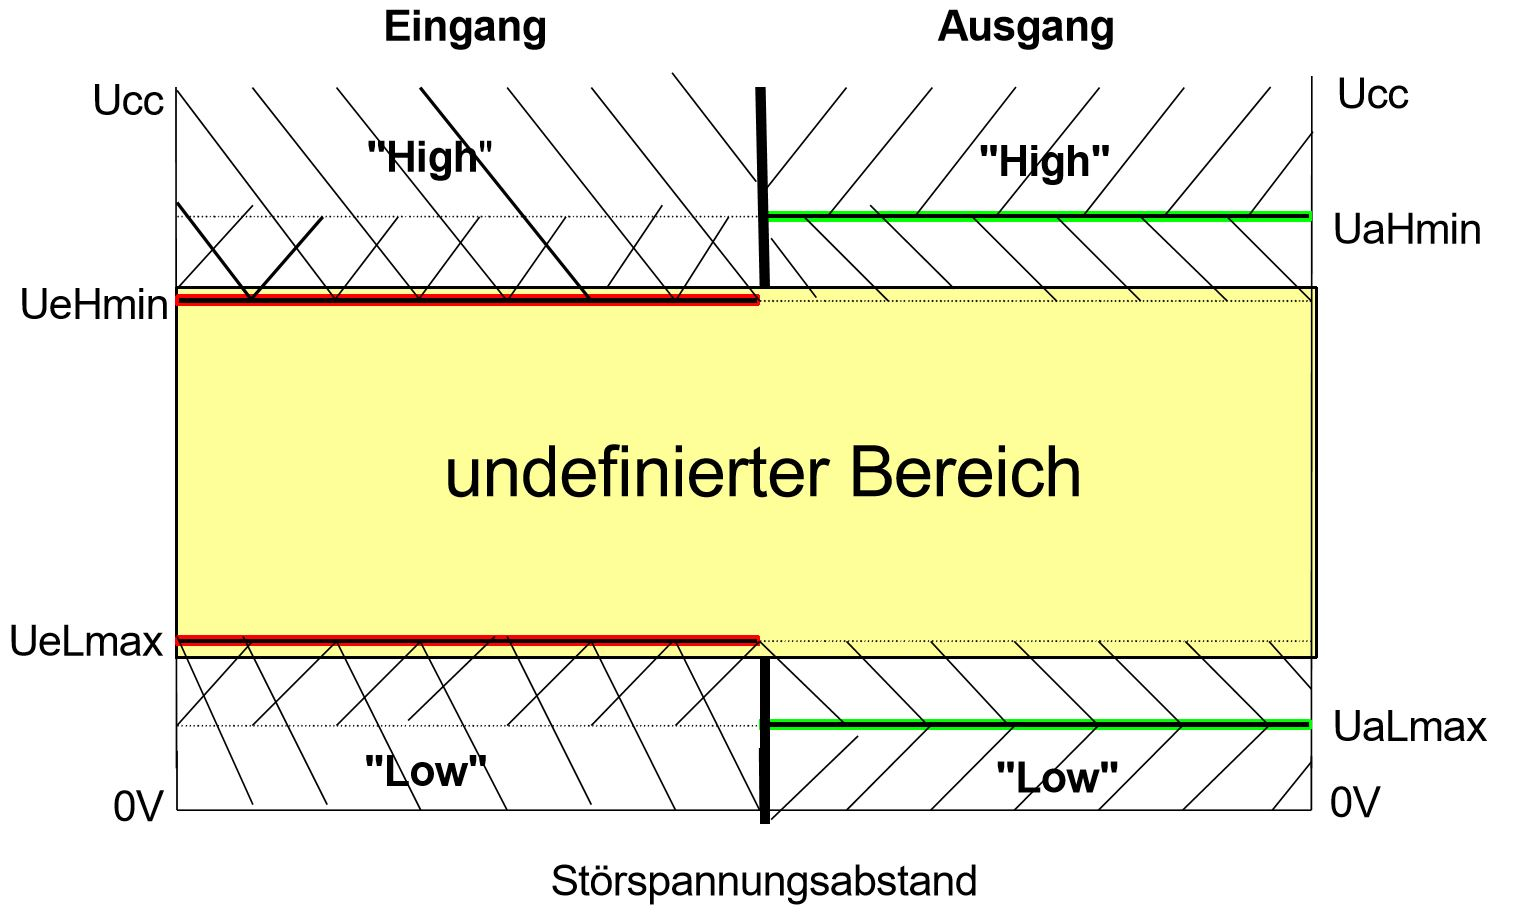
\includegraphics[width=0.8\textwidth]{./1_1_Z1.jpg}
      \end{center}
    \end{figure}

    $\spannung{U_{eH_{min}}}$; $\spannung{U_{aH_{max}}}$: mindestens oder "`Worst-Case"'-Pegel für Logik. "`1"'\\
    $\spannung{U_{eL_{min}}}$; $\spannung{U_{aL_{max}}}$: maximaler oder "`Worst-Case"'-Pegel für Logik. "`0"'\\
    $\spannung{U_{cc}}$ = Versorgungsspannung\\

    \section{Vorbereitungsaufgaben}

      \paragraph{Aufgabe 1:} Was versteht man unter dem Gleichspannungs - Störabstand bei logischen Schaltungen? Wie berechnet man ihn? Bsp. für LS-TTL-Logik angeben.

      

      \paragraph{Aufgabe 2:} Berechnen Sie die Werte der Störabstände in der unten aufgeführten Tabelle.\\
        Annahme: $\spannung{U_{cc}} = \SI{4,5}{\volt}$

      \paragraph{Aufgabe 3:} Tragen Sie die fehlenden Werte in die Tabelle ein:

        \begin{center}
          \begin{table}[H]
            \caption{Kenngrössen verschiedener Logikfamilien}
              \label{tbl:Kenngroessen}
              \renewcommand{\arraystretch}{1.6}
              \begin{center}
                \begin{tabular}{c| c|c|c}
                  & LS-TTL & HCHMOS & Advanced CMOS\\
                  Versorg.-Spg. $\spannung{U_{CC}}$ & \qquad\qquad\qquad & \SI{2}{\volt} - \SI{6}{\volt} & \SI{2}{\volt} - \SI{6}{\volt}\\ \hline
                  Eingangspegel &\qquad\qquad\qquad&\qquad\qquad\qquad&\qquad\qquad\qquad\\ 
                  & &  & \\ \hline
                  $\spannung{U_{eHmin}}$&&&\\ \hline
                  Ausgangspegel:&&& \\
                  $\spannung{U_{aLmax}}$&&& \\ \hline
                  $\spannung{U_{aHmin}}$&&&\\ \hline
                  Störabstand &&&\\ 
                  "`Low"' & & & \\ \hline
                  "`High"' & & & \\ \hline
                  Arbeitstemperatur & \qquad\si{\degreeCelsius} -- \qquad\si{\degreeCelsius} & \qquad\si{\degreeCelsius} -- \qquad\si{\degreeCelsius} & \qquad\si{\degreeCelsius} -- \qquad\si{\degreeCelsius}
                \end{tabular}
              \end{center}
          \end{table}
        \end{center}

      \paragraph{Eingangsspannungsvorgabe:}

        \begin{center}
          \begin{circuitikz}[scale=1]
            \draw
              (0,4) to[short] (3,4)
                    to[short, -o] (4,4)
              (0,0) to[short] (3,0)
                    to[short, -o] (4,0)

              (0,4) to[R, l=\SI{2,2}{\kilo\ohm}, -*] (0,2)
                    to[R, l=\SI{330}{\ohm}] (0,0)

              (2,4) to[R, l=\SI{2,2}{\kilo\ohm}, -*] (2,2)
                    to[R, l=\SI{1,5}{\kilo\ohm}] (2,0)



              (5.2,4) node{$\spannung{U_{cc}} = \SI{5,2}{\volt}$}
              (4.5,0) node{$\SI{0}{\volt}$}
            ;
            \path[->, blue](0,2) edge node[auto] {$\spannung{U_{eL}}$} (-1.5,2);
            \path[->, blue](2,2) edge node[auto] {$\spannung{U_{eH}}$} (3.5,2);
          \end{circuitikz}
        \end{center}

    \section{Wertetabelle NAND-Gatter}
      Messen Sie die Wertetabelle eines NAND-Gatters (74LS00), indem Sie die Ein- und
      Ausgangsspannungen protokollieren.

      \begin{center}
        \begin{table}[!hbtp]
          \caption{Wertetabelle NAND-Gatter}
          \renewcommand{\arraystretch}{1.6}
          \begin{center}
            \begin{tabular}{c|c|c}
              $\spannung{U_a} [\si{\volt}]$ & $\spannung{U_b} [\si{\volt}]$ & $\spannung{U_y} [\si{\volt}]$ \\ \hline
               & &\\\hline
               &  &\\\hline
              &  &\\\hline
              && \\
            \end{tabular}
          \end{center}
        \end{table}
      \end{center}

    \section{Übertragungskennlinie eines TTL-Gatters}
      \paragraph{Vorbereitungsaufgabe:}Wie wird bei einem TTL- Gatter ein unbeschalteter Eingang interpretiert? Begründen Sie dieses.


      \paragraph{Messschaltung:}
        \begin{center}
          \begin{circuitikz}[scale=1]
          \ctikzset{label/align = rotate}
            \draw
              (2.5,1.5) node[label={[shift={(0.25,-0.35)}]\texttt{\scriptsize E1}}](E1){}
              (2.5,2.5) node[label={[shift={(0.25,-0.35)}]\texttt{\scriptsize E2}}](E2){}
              (3.5,2) node[label={[shift={(-0.25,-0.35)}]\texttt{\scriptsize A}}](A){}
              (3,1) node[label={[shift={(0,-0.2)}]\texttt{\scriptsize GND}}](GND){}
              (3,3.5) node[label={[shift={(0,-1)}]\texttt{\scriptsize Vcc}}](V){}
              (2.9,2) node{\texttt{\textbf \&}}
              (3.7,3.15) node{\texttt{\scriptsize 74LS00}}
              (6,4) node{$\spannung{U_{CC}} = \SI{5}{\volt}$}
              (5.5,0) node{$\SI{0}{\volt}$}

              (0,0) to[short, -o] (5,0)
              (0,4) to[short, -o] (5,4)
              (3,0) to[short, *-] (3,1)
              (3,4) to[short, *-] (3,3)
              (2.5,1) rectangle (3.5,3)
              (1.5,4) to[short, *-] (1.5,2 |- E1)
                      to[short] (E1)

              (A) to[short, -o] (4,3 |-A)
                  to[open, v^=$\spannung{U_a}$] (4,0)

              (0,4) to[pR] (0,1)
              (0.5,2.5) to[short] (E2)
              (0,1) to[short] (0,0)

              (1,2.5) to[open, v=$\spannung{U_e}$] (1,0)
            ;
          \end{circuitikz}
        \end{center}


      \subsection{Messaufgaben}
        \paragraph{Messaufgabe M1:} Übertragungskennlinie $\spannung{U_a} = f(\spannung{U_e})$ eines TTL- Gatters (74LS00) aufnehmen.\\
          Vorgaben / Einstellungen:\\
          Versorgungsspannung $\spannung{U_{cc}} = \SI{5}{\volt}$\\
          Eingangsspannung $\spannung{U_e}$ nach Tabelle 1.3 vorgegeben.

          \begin{center}
            \begin{table}[H]
              \caption{Messwerte Messaufgabe 1}
              \renewcommand{\arraystretch}{1.6}
              \begin{center}
                \begin{tabular}{c|c}
                  $\spannung{U_e} [\si{\volt}]$ & $\spannung{U_a} [\si{\volt}]$ \\ \hline
                   0,2& \qquad\qquad\qquad\qquad\\\hline
                   0,4& \\\hline
                   0,8& \\\hline
                   0,9& \\\hline
                   1,0& \\\hline
                   1,1& \\\hline
                   1,2& \\\hline
                   1,3& \\\hline
                   1,4&
                \end{tabular}
              \end{center}
            \end{table}
          \end{center}

        \paragraph{Messaufgabe M2:} Ermitteln Sie die Schaltschwelle Uth. Verbinden Sie dazu einen Eingang mit dem Ausgang des Gatters.

          \begin{equation*}
            \spannung{U_{th}} =
          \end{equation*}

          \begin{center}
            \begin{circuitikz}[scale=1]
              \ctikzset{label/align = rotate}
              \draw
                (2.5,1.5) node[label={[shift={(0.25,-0.35)}]\texttt{\scriptsize E1}}](E1){}
                (2.5,2.5) node[label={[shift={(0.25,-0.35)}]\texttt{\scriptsize E2}}](E2){}
                (3.5,2) node[label={[shift={(-0.25,-0.35)}]\texttt{\scriptsize A}}](A){}
                (3,1) node[label={[shift={(0,-0.2)}]\texttt{\scriptsize GND}}](GND){}
                (3,3.5) node[label={[shift={(0,-1)}]\texttt{\scriptsize Vcc}}](V){}
                (2.9,2) node{\texttt{\textbf \&}}
                (3.7,3.15) node{\texttt{\scriptsize 74LS00}}
                (6,4) node{$\spannung{U_{CC}} = \SI{5}{\volt}$}
                (5.5,0) node{$\SI{0}{\volt}$}

                (0,0) to[short, -o] (5,0)
                (0,4) to[short, -o] (5,4)
                (3,0) to[short, *-] (3,1)
                (3,4) to[short, *-] (3,3)
                (2.5,1) rectangle (3.5,3)


                (A) to[short] (4,3 |-A)
                    to[short] (4,0.5)
                    to[short] (2,0.5)
                    to[short] (2,2 |-E1)
                    to[short] (E1)
                (4,3 |-A) to[open, v^=$\spannung{U_a}$] (4,0)

                (0,4) to[pR] (0,1)
                (0.5,2.5) to[short] (E2)
                (0,1) to[short] (0,0)

                (1,2.5) to[open, v=$\spannung{U_e}$] (1,0)
              ;
            \end{circuitikz}
          \end{center}

      \subsection{Auswertung}
        \paragraph{Auswertung A1:} Zeichnen Sie die Kennlinie.


        \paragraph{Auswertung A2:} Ermitteln Sie aus der Übertragungskennlinie:\\
          a) Schaltschwelle(Umschaltspannung) $\spannung{U_{th}}$\\
          b) Kurvenpunkt mit der Verstärkung dUa/dUe = 1; A1 (UeLmax, UaHmin), A2 (UeHmin, UaLmax).

        a) $\spannung{U_{th}} = \SI{1,01}{\volt}$\\
        b) Der Kurvenpunkt entspricht dem Punkt bei $\spannung{U_{th}}$

        \paragraph{Auswertung A3:}\label{sec:auswertung-a3} Warum kann die Schaltschwelle $\spannung{U_{th}}$ bei invertierenden Gattern durch Zusammenschalten von Ein- und Ausgang ermittelt werden?

        \paragraph{Auswertung A4:} Warum weichen die ermittelten Kenngrößen von den Datenblattangaben ab?

    \chapter{Belastung logischer Schaltungen}
      \paragraph{Vorbereitungsaufgaben:} Was versteht man unter:\\
        a) Ausgangslastfaktor ("`fan-out"')\\
        b) Eingangslastfaktor ("`fan-in"')

        
    \section{Übung 1: Eingangskennlinie $I_e = f(U_e)$ eines TTL-Gatters}
      \paragraph{Messschaltung:}
        \begin{center}
          \begin{circuitikz}[scale=1]
            \ctikzset{label/align = rotate}
            \draw
              (2.5,1.5) node[label={[shift={(0.25,-0.35)}]\texttt{\scriptsize E1}}](E1){}
              (2.5,2.5) node[label={[shift={(0.25,-0.35)}]\texttt{\scriptsize E2}}](E2){}
              (3.5,2) node[label={[shift={(-0.25,-0.35)}]\texttt{\scriptsize A}}](A){}
              (3,1) node[label={[shift={(0,-0.2)}]\texttt{\scriptsize GND}}](GND){}
              (3,3.5) node[label={[shift={(0,-1)}]\texttt{\scriptsize Vcc}}](V){}
              (2.9,2) node{\texttt{\textbf \&}}
              (3.7,3.15) node{\texttt{\scriptsize 74LS00}}
              (6,4) node{$\spannung{U_{CC}} = \SI{5}{\volt}$}
              (5.5,0) node{$\SI{0}{\volt}$}

              (0,0) to[short, -o] (5,0)
              (0,4) to[short, -o] (5,4)
              (3,0) to[short, *-] (3,1)
              (3,4) to[short, *-] (3,3)
              (2.5,1) rectangle (3.5,3)
              (1.5,4) to[short, *-] (1.5,2 |- E1)
                      to[short] (E1)

              (A) to[short, -o] (4,3 |-A)

              (0,4) to[pR] (0,1)
              (0.5,2.5) to[short, i=$\strom{I_e}$] (E2)
              (0,1) to[short] (0,0)

              (1,2.5) to[open, v=$\spannung{U_e}$] (1,0)
            ;
          \end{circuitikz}
        \end{center}



      \subsection{Messaufgaben}
        \paragraph{Messaufgabe M1:} Nehmen Sie die Eingangskennlinie $\strom{I_e} = f(\spannung{U_e})$ eines TTL- Gatters 74LS00 auf. Eingangsspannung mit Potentiometer vorgeben.
            \begin{center}
                \begin{table}[H]
                    \caption{Messwerte Messaufgabe 1}
                    \renewcommand{\arraystretch}{1.6}
                    \begin{center}
                        \begin{tabular}{c|c}
                            $\spannung{U_e} [\si{\volt}]$ & $\strom{I_e} [\si{\micro\ampere}]$ \\ \hline
                            0,2 & \qquad\qquad\qquad\qquad\\\hline
                            0,4 & \\\hline
                            0,8 & \\\hline
                            1,0 & \\\hline
                            2,0 & \\\hline
                            2,4 & \\\hline
                            2,7 & \\\hline
                            3,0 & \\\hline
                            5,0 & \\
                        \end{tabular}
                    \end{center}
                \end{table}
            \end{center}


      \subsection{Auswertung}
        \paragraph{Auswertung A1:} Stellen Sie die Eingangkennlinie graphisch dar.


        \paragraph{Auswertung A2:} Wie groß sind die Eingangsströme bei den "`Worst-Case"' Eingangsspannungen?

          \begin{center}
            \begin{table}[H]
              \caption{"'Worst-Case"' Eingangsströme}
              \renewcommand{\arraystretch}{1.6}
              \begin{center}
                \begin{tabular}{c|c|c}
                  &$\spannung{U_e} [\si{\volt}]$ & $\strom{I_e} [\si{\milli\ampere}]$\\\hline
                  "`Worst-Case"' LOW & \qquad\qquad\qquad\qquad & \qquad\qquad\qquad\qquad\\\hline
                  "`Worst-'Case"' HIGHT& & \\
                \end{tabular}
              \end{center}
            \end{table}
          \end{center}

    \section{Übung 2: Ausgangskennlinie eines TTL-Gatters (74LS00)}
      \paragraph{Messschaltung:}
      \paragraph{Messschaltung $U_A$ = "`low"':}

        \begin{center}
        \begin{circuitikz}[scale=1]
        \draw
          (2.5,1.5) node[label={[shift={(0.25,-0.35)}]\texttt{\scriptsize E1}}](E1){}
          (2.5,2.5) node[label={[shift={(0.25,-0.35)}]\texttt{\scriptsize E2}}](E2){}
          (3.5,2) node[label={[shift={(-0.25,-0.35)}]\texttt{\scriptsize A}}](A){}
          (3,1) node[label={[shift={(0,-0.2)}]\texttt{\scriptsize GND}}](GND){}
          (3,3.5) node[label={[shift={(0,-1)}]\texttt{\scriptsize Vcc}}](V){}
          (2.9,2) node{\texttt{\textbf \&}}
          (2.3,3.15) node{\texttt{\scriptsize 74LS00}}
          (7,6) node{$\spannung{U_{CC}} = \SI{5}{\volt}$}
          (6.5,0) node{$\SI{0}{\volt}$}

          (3,0) to[short, -o] (6,0)
          (3,6) to[short, -o] (6,6)
          (3,0) to[short] (3,1)
          (3,6) to[short] (3,3)
          (2.5,1) rectangle (3.5,3)

          (A) to[short] (5,2 |-A)
              to[pR, l_=\SI{4,7}{\kilo\ohm}] (5,4.5)
              to[R, l_=\SI{51}{\ohm}] (5,6)
          (4.45,3.25) to[short, i_=$\strom{I_a}$] (4.45,2 |-A)
                      to[open, v=$\spannung{U_a}$] (4.45,0)
        ;
        \end{circuitikz}
        \end{center}

      \paragraph{Messschaltung $U_A$ = "`high"':}

        \begin{center}
          \begin{circuitikz}[scale=1]
            \draw
              (2.5,1.5) node[label={[shift={(0.25,-0.35)}]\texttt{\scriptsize E1}}](E1){}
              (2.5,2.5) node[label={[shift={(0.25,-0.35)}]\texttt{\scriptsize E2}}](E2){}
              (3.5,2) node[label={[shift={(-0.25,-0.35)}]\texttt{\scriptsize A}}](A){}
              (3,1) node[label={[shift={(0,-0.2)}]\texttt{\scriptsize GND}}](GND){}
              (3,3) node[label={[shift={(0,-0.5)}]\texttt{\scriptsize Vcc}}](V){}
              (2.9,2) node{\texttt{\textbf \&}}
              (2.3,3.15) node{\texttt{\scriptsize 74LS00}}
              (4,3.5) node{$\spannung{U_{CC}} = \SI{5}{\volt}$}
              (7.5,-2) node{$\SI{0}{\volt}$}

              (3,-2) to[short, -o] (7,-2)
              (V) to[short, -o] (4,3.5 -|V)
              (3,-2) to[short, *-] (3,1)
              (2.5,1) rectangle (3.5,3)

              (A) to[short, i=$\strom{I_a}$] (5,3 |-A)
                  to[R, l=\SI{51}{\ohm}](5,0)
                  to[pR, l=\SI{4,7}{\kilo\ohm}, -*] (5,-2)
              (5.55,-2) to[short, *-] (5.55,-1)

              (3,-2) to[short] (2,-2)
                    to[short] (2,3 |-E1)
                    to[short] (E1)

              (4,3 |-A) to[open, v=$\spannung{U_a}$] (4,-2)
            ;
          \end{circuitikz}
        \end{center}

      \subsection{Messaufgaben}
        \paragraph{Messaufgabe M1:} Nehmen Sie die Ausgangskennlinie $\spannung{U_a} = f(\strom{I_a})$ eines TTL(Transistor/ Transistor Logik)-Gatters 74LS00 für low und für high-Pegel auf.\\
          Vorgaben/Einstellungen:\\
          Versorgungsspannung $\spannung{U_{cc}} = \SI{5}{\volt}$\\
          Ausgang stufenweise, durch Ändern des Potentiometerwiderstandes, belasten.

          \begin{center}
            \begin{table}[H]
              \caption{Messwerte Messaufgabe 1}
              \renewcommand{\arraystretch}{1.6}
              \begin{center}
                \begin{tabular}{c|c|c|c|c}
                  \multicolumn{2}{c|}{"'Low"' Pegel am Ausgang} &&\multicolumn{2}{c}{"'High"' Pegel am Ausgang}\\
                  $\spannung{U_a} [\si{\volt}]$ & $\strom{I_a} [\si{\milli\ampere}] $&& $\spannung{U_a} [\si{\volt}]$ & $\strom{I_a} [\si{\milli\ampere}] $\\ \hline
                  \qquad\qquad\qquad\qquad & \qquad\qquad\qquad\qquad &  & \qquad\qquad\qquad\qquad & \qquad\qquad\qquad\qquad\\\hline
                   &  &  &  & \\\hline
                   &  &  &  & \\\hline
                   &  &  &  & \\\hline
                   &  &  &  & \\\hline
                   &  &  &  & \\\hline
                   &  &  &  & \\\hline
                   &  &  &  & \\\hline
                   &  &  &  & \\\hline
                   &  &  &  & \\\hline
                   &  &  & &
                \end{tabular}
              \end{center}
            \end{table}
          \end{center}


      \subsection{Auswertung}
        \paragraph{Auswertung A1:} Stellen Sie die Ausgangskennlinien graphisch dar($\spannung{U_a} = f(\strom{I_a})$).


        \paragraph{Auswertung A2:} Bestimmen Sie in LS-TTL- Einheiten:\\
          a) den maximalen Ausgangslastfaktor aus der Ausgangskennlinie $\spannung{U_a} = f(\strom{I_a})$ und der Eingangskennlinie $\strom{I_e} = f(\spannung{U_e})$ (High und Low)\\
          b) den zulässigen (empfohlenen) Ausgangslastfaktor aus den Datenblattangaben.
          Warum ist es nicht ratsam ein Gatter mit dem maximal möglichem fan-out zu belasten?

        
             
  \chapter{Schaltzeiten von TTL-Gattern}
    \paragraph{Vorbereitungsaufgaben:} Erklären Sie:\\a) Anstiegszeit \textbf{$t_r$}\\b) Abfallzeit \textbf{$t_f$}

    
    \section{Übung 1: Schaltzeiten eines TTL-Gatters (74LS00)}
      Bei der Realisierung von taktgesteuerten Funktionseinheiten kommt des öfteren eine sogenannte spike-Schaltung zum Einsatz. Die hier vorgestellte Schaltung nutzt zur Impulserzeugung die Gatterlaufzeit aus.
      
      \paragraph{Messschaltung: Spike-Schaltung:}
        \begin{center}
            \begin{circuitikz}[scale=1]
                \ctikzset{label/align = rotate}
                
                % Gatter 1
                \node at (1,8.5) (g1) {};
                \draw
                (g1) rectangle ($(g1) + (1,2)$)
                ($(g1) + (0,0.5)$) node[label={[shift={(0.25,-0.35)}]\texttt{\scriptsize E1}}](1E1){}
                ($(g1) + (0,1.5)$) node[label={[shift={(0.25,-0.35)}]\texttt{\scriptsize E2}}](1E2){}
                ($(g1) + (1,1)$) node[label={[shift={(-0.25,-0.35)}]\texttt{\scriptsize A}}](1A){}
                ($(g1) + (0.5,0)$) node[label={[shift={(0,-0.2)}]\texttt{\scriptsize GND}}](1GND){}
                ($(g1) + (0.5,2)$) node[label={[shift={(0,-0.5)}]\texttt{\scriptsize Vcc}}](1V){}
                ($(g1) + (0.4,1)$) node{\texttt{\textbf \&}}
                ($(g1) + (1,2.2)$) node{\texttt{\scriptsize N1/1}}
                ;
                % Gatter 2
                \node at ($(1A) + (1,-1.5)$) (g2) {};
                \draw
                (g2) rectangle ($(g2) + (1,2)$)
                ($(g2) + (0,0.5)$) node[label={[shift={(0.25,-0.35)}]\texttt{\scriptsize E1}}](2E1){}
                ($(g2) + (0,1.5)$) node[label={[shift={(0.25,-0.35)}]\texttt{\scriptsize E2}}](2E2){}
                ($(g2) + (1,1)$) node[label={[shift={(-0.25,-0.35)}]\texttt{\scriptsize A}}](2A){}
                ($(g2) + (0.5,0)$) node[label={[shift={(0,-0.2)}]\texttt{\scriptsize GND}}](2GND){}
                ($(g2) + (0.5,2)$) node[label={[shift={(0,-0.5)}]\texttt{\scriptsize Vcc}}](2V){}
                ($(g2) + (0.4,1)$) node{\texttt{\textbf \&}}
                ($(g2) + (1,2.2)$) node{\texttt{\scriptsize N1/2}}
                ;
                
                % Gatter 3
                \node at ($(2A) + (1,-1.5)$) (g3) {};
                \draw
                (g3) rectangle ($(g3) + (1,2)$)
                ($(g3) + (0,0.5)$) node[label={[shift={(0.25,-0.35)}]\texttt{\scriptsize E1}}](3E1){}
                ($(g3) + (0,1.5)$) node[label={[shift={(0.25,-0.35)}]\texttt{\scriptsize E2}}](3E2){}
                ($(g3) + (1,1)$) node[label={[shift={(-0.25,-0.35)}]\texttt{\scriptsize A}}](3A){}
                ($(g3) + (0.5,0)$) node[label={[shift={(0,-0.2)}]\texttt{\scriptsize GND}}](3GND){}
                ($(g3) + (0.5,2)$) node[label={[shift={(0,-0.5)}]\texttt{\scriptsize Vcc}}](3V){}
                ($(g3) + (0.4,1)$) node{\texttt{\textbf \&}}
                ($(g3) + (1,2.2)$) node{\texttt{\scriptsize N1/3}}
                ;
                
                
                % Gatter 4
                \node at ($(3A) + (1,-1.5)$) (g4) {};
                \draw
                (g4) rectangle ($(g4) + (1,2)$)
                ($(g4) + (0,0.5)$) node[label={[shift={(0.25,-0.35)}]\texttt{\scriptsize E1}}](4E1){}
                ($(g4) + (0,1.5)$) node[label={[shift={(0.25,-0.35)}]\texttt{\scriptsize E2}}](4E2){}
                ($(g4) + (1,1)$) node[label={[shift={(-0.25,-0.35)}]\texttt{\scriptsize A}}](4A){}
                ($(g4) + (0.5,0)$) node[label={[shift={(0,-0.2)}]\texttt{\scriptsize GND}}](4GND){}
                ($(g4) + (0.5,2)$) node[label={[shift={(0,-0.5)}]\texttt{\scriptsize Vcc}}](4V){}
                ($(g4) + (0.4,1)$) node{\texttt{\textbf \&}}
                ($(g4) + (1,2.2)$) node{\texttt{\scriptsize N1/4}}
                ;
                
                \draw
                
                 % Ground and Squarewave
                ($(1E2) - (-8,4)$) node[ground]{}
                ($(1E2) - (0.5,0)$) to[short] (1E2)
                ($(1E2) - (2,0)$) to[sqV, l=\SI{1}{\mega\hertz}] ($(1E2) - (0.5,0)$)
                ($(1E2) - (2,0)$) to[short] ($(1E2) - (2,4)$)
                                  to[short] ($(1E2) - (-8,4)$)
                (1GND) to[short, -*]  ($(1GND) - (0,2.5)$)
                (2GND) to[short, -*]  ($(2GND) - (0,2)$)
                (3GND) to[short, -*]  ($(3GND) - (0,1.5)$)
                (4GND) to[short, -*]  ($(4GND) - (0,1)$)
                  
                % Spannungsversorgung                
                ($(1V) + (8,1)$) node{$\spannung{U_{CC}} = \SI{5}{\volt}$}
                ($(1V) + (0,1)$) to[short, -o] ($(1V) + (7,1)$)
                (1V) to[short] ($(1V) + (0,1)$)
                (2V) to[short, -*] ($(2V) + (0,1.5)$)
                (3V) to[short, -*] ($(3V) + (0,2)$)
                (4V) to[short, -*] ($(4V) + (0,2.5)$)                  
                                                
                (1A) to[short, l=$X_1$] (2E2)
                (2A) to[short, l=$X_2$] (3E2)
                (3A) to[short, l=$X_3$] (4E2)
                (4A) to[short, l=$X_4$] ($(4A) + (1,0)$)
                     to[short] ($(4A) + (1,-1.5)$)
                     to[short] ($(4A) + (0,-1.5)$)
                     to[short, -*] ($(4A) + (0,-2)$)
                
                ($(1E2) - (0.5,0)$) to[short, *-] ($(1E2) - (0.5,3)$)
                                    to[short] ($(4E1) - (0.5,0.5)$)
                                    to[short] ($(4E1) - (0.5,0)$)
                                    to[short] (4E1)
                                    

                ;
            \end{circuitikz}
        \end{center}

      Vorgaben/Einstellungen:
      \begin{itemize*}
        \item Zum Messen die Tastköpfe benutzen und Masseleitung anschließen
        \item Versorgungsspannung $\spannung{U_{cc}} = \SI{5}{\volt}$
        \item Eingangssignal an X0 mit dem Frequenzgenerator vorgeben: $f = \SI{1}{\mega\Hz}$; TTL-Ausgang verwenden, wenn vorhanden!
        \item Schaltung aufbauen
        \item Leitungsführung kurz halten
      \end{itemize*}

      \subsection{Messaufgaben}
        \paragraph{Messaufgabe M1:} Messen Sie die Signalverläufe von X1 und X2 mit dem Oszillograph. Bestimmen Sie:

          Anstiegszeit $t_r$ von $X_2$: \\
          Abfallzeit $t_f$ von $X_2$: 

          Signallaufzeiten für Gatter N1/2:\\
          $t_{pHL}$ (Ausgang high nach low): \\
          $t_{pLH}$ (Ausgang low nach high): \\

          Tragen Sie die Signalverläufe X1 und X2 in ein zu erstellendes Zeitdiagramm ein.


        \paragraph{Messaufgabe M2:} Messen Sie die Signalverläufe von X1 und X4 mit dem Oszillograph und stellen Sie die
          Signalverläufe graphisch mit Zeitangabe (farbig) dar.

      \subsection{Auswertung}
        \paragraph{Zwischenaufgabe:} Wie viele Ic's werden benötigt?
                
        \paragraph{Auswertung A1:} Vergleichen Sie die Messwerte mit den im Datenblatt angegebenen und erklären Sie
        eventuelle Abweichungen.


  \chapter{Impuls-Schaltung}
    \section{Übung 1}
      \paragraph{Messschaltung:}

       \begin{center}
           \begin{circuitikz}[scale=1]
               \ctikzset{label/align = rotate}
               
               % Gatter 1
               \node at (1,8.5) (g1) {};
               \draw
               (g1) rectangle ($(g1) + (1,2)$)
               ($(g1) + (0,0.5)$) node[label={[shift={(0.25,-0.35)}]\texttt{\scriptsize E1}}](1E1){}
               ($(g1) + (0,1.5)$) node[label={[shift={(0.25,-0.35)}]\texttt{\scriptsize E2}}](1E2){}
               ($(g1) + (1,1)$) node[label={[shift={(-0.25,-0.35)}]\texttt{\scriptsize A}}](1A){}
               ($(g1) + (0.5,0)$) node[label={[shift={(0,-0.2)}]\texttt{\scriptsize GND}}](1GND){}
               ($(g1) + (0.5,2)$) node[label={[shift={(0,-0.5)}]\texttt{\scriptsize Vcc}}](1V){}
               ($(g1) + (0.4,1)$) node{\texttt{\textbf \&}}
               ($(g1) + (1,2.2)$) node{\texttt{\scriptsize N1/1}}
               ;
               % Gatter 2
               \node at ($(g1) + (4,0)$) (g2) {};
               \draw
               (g2) rectangle ($(g2) + (1,2)$)
               ($(g2) + (0,0.5)$) node[label={[shift={(0.25,-0.35)}]\texttt{\scriptsize E1}}](2E1){}
               ($(g2) + (0,1.5)$) node[label={[shift={(0.25,-0.35)}]\texttt{\scriptsize E2}}](2E2){}
               ($(g2) + (1,1)$) node[label={[shift={(-0.25,-0.35)}]\texttt{\scriptsize A}}](2A){}
               ($(g2) + (0.5,0)$) node[label={[shift={(0,-0.2)}]\texttt{\scriptsize GND}}](2GND){}
               ($(g2) + (0.5,2)$) node[label={[shift={(0,-0.5)}]\texttt{\scriptsize Vcc}}](2V){}
               ($(g2) + (0.4,1)$) node{\texttt{\textbf \&}}
               ($(g2) + (1,2.2)$) node{\texttt{\scriptsize N1/2}}
               ;
               
               % Gatter 3
               \node at ($(g2) + (2,0)$) (g3) {};
               \draw
               (g3) rectangle ($(g3) + (1,2)$)
               ($(g3) + (0,0.5)$) node[label={[shift={(0.25,-0.35)}]\texttt{\scriptsize E1}}](3E1){}
               ($(g3) + (0,1.5)$) node[label={[shift={(0.25,-0.35)}]\texttt{\scriptsize E2}}](3E2){}
               ($(g3) + (1,1)$) node[label={[shift={(-0.25,-0.35)}]\texttt{\scriptsize A}}](3A){}
               ($(g3) + (0.5,0)$) node[label={[shift={(0,-0.2)}]\texttt{\scriptsize GND}}](3GND){}
               ($(g3) + (0.5,2)$) node[label={[shift={(0,-0.5)}]\texttt{\scriptsize Vcc}}](3V){}
               ($(g3) + (0.4,1)$) node{\texttt{\textbf \&}}
               ($(g3) + (1,2.2)$) node{\texttt{\scriptsize N1/3}}
               ;
               
               
               \draw
               
               % Ground and Squarewave
               ($(1E2) - (-8,4)$) node[ground]{}
               ($(1E2) - (0.5,0)$) to[short] (1E2)
               ($(1E2) - (2,0)$) to[sqV, l=\SI{500}{\hertz}] ($(1E2) - (0.5,0)$)
               ($(1E2) - (2,0)$) to[short] ($(1E2) - (2,4)$)
               to[short] ($(1E2) - (-8,4)$)
               (1GND) to[short, -*]  ($(1GND) - (0,2.5)$)
               (2GND) to[short, -*]  ($(2GND) - (0,2.5)$)
               (3GND) to[short, -*]  ($(3GND) - (0,2.5)$)
               
               % Spannungsversorgung                
               ($(1V) + (8,1)$) node{$\spannung{U_{CC}} = \SI{5}{\volt}$}
               ($(1V) + (0,1)$) to[short, -o] ($(1V) + (7,1)$)
               (1V) to[short] ($(1V) + (0,1)$)
               (2V) to[short, -*] ($(2V) + (0,1)$)
               (3V) to[short, -*] ($(3V) + (0,1)$)
               
               
               %($(1E2) - (0.5,0)$) to[short, *-] ($(1E2) - (0.5,3)$)
               %to[short] ($(4E1) - (0.5,0.5)$)
               %to[short] ($(4E1) - (0.5,0)$)
               %to[short] (4E1)
               
               %Condensator Stuff
               (1A) to[R, l=\SI{2,2}{\kilo\ohm}] ($(1A) + (1.5,0)$)
                    to[C, *-*, l=\SI{0,022}{\micro\farad}] ($(1A) + (1.5,-3.5)$)
               ($(1A) + (1.5,0)$) to[short, l=$X_1$] (2E1)
               
               %split N2
               (2A) to[short, -*, l=$X_2$] ($(2A) + (0.5,0)$)
               ($(2A) + (0.5,0)$) to[short] (3E1)  
               ($(2A) + (0.5,0)$) to[short] (3E2)
               
               %Frequenzgeneratro Hook up
               ($(1E2) - (0.5,0)$) to[short, *-] ($(1E2) - (0.5,1)$)
                                   to[short] (1E1)
               ($(1E2) - (0.5,0)$) to[short] ($(1E2) - (0.5,-1)$)
                                   to[short] ($(2E2) + (-0.5,1)$)
                                   to[short, l=$X_0$] ($(2E2) + (-0.5,0)$)
                                   to[short] (2E2)
                                   
              %Zeug
              (3A) to[short, l=$X_3$] ($(3A)+(1,0)$)
                   to[short, -*] ($(3A)+(1,-3.5)$)
               ;
           \end{circuitikz}
       \end{center}
        Vorgaben/Einstellungen:\\
        Versorgungsspannung $\spannung{U_{cc}} = \SI{5}{\volt}$ und Eingangssignal X0 mit dem Frequenzgenerator auf $f = \SI{500}{\Hz}$ einstellen; TTL-Ausgang verwenden!

      \subsection{Messaufgaben}
        \paragraph{Messaufgabe M1:} Messen Sie die Signale X0, X1 und X3 der Schaltung mit dem Oszillograph. Stellen Sie die Signalverläufe von X0, X1 und X3 in einer Zeichnung untereinander da.

        \paragraph{Messaufgabe M2:} Erklären Sie den Begriff Impulsdauer. Wie groß ist hier die Impulsdauer $t_i$ des Ausgangssignals?

        \paragraph{Messaufgabe M3:} Bestimmen Sie die Schaltschwelle $\spannung{U_{th}}$ des Gatters N1/2:

      \subsection{Auswertung}
        \paragraph{Auswertung A1:} Beschreiben Sie die Funktionsweise der Schaltung mit Zeitablaufdiagramm und Funktionstabelle.
        
          
        \paragraph{Auswertung A2:} Geben Sie eine Formel zur Berechnung der Impulsdauer $t_i = f(\widerstand{R}, \capacity{C}, \spannung{U_e})$ an.

        \paragraph{Auswertung A3:} Berechnen Sie $t_i$ für obige Schaltung; Rechnen Sie mit der zuvor gemessenen
          Schaltschwelle $\spannung{U_{eth}}$. Vergleichen Sie das Ergebnis mit der Messung.

        
  \chapter{Flip-Flop-Speicher}
    \section{Übung 1: RS-Flip-Flop}
      Ergänzen Sie nachfolgende Schaltung mit einem RS-Flip-Flop, aufgebaut aus NAND-Gattern.\\
      Für die Eingänge des 'R'S- FF' gilt:\\
      Setzen: S = 0\\
      Rücksetzen: R = 0 
         \begin{center}
            \begin{circuitikz}[scale=1]
                \ctikzset{label/align = rotate}
                
                % Gatter 1
                \node at (1,8.5) (g1) {};
                \draw
                (g1) rectangle ($(g1) + (1,2)$)
                ($(g1) + (0,0.5)$) node[label={[shift={(0.25,-0.35)}]\texttt{\scriptsize E1}}](1E1){}
                ($(g1) + (0,1.5)$) node[label={[shift={(0.25,-0.35)}]\texttt{\scriptsize E2}}](1E2){}
                ($(g1) + (1,1)$) node[label={[shift={(-0.25,-0.35)}]\texttt{\scriptsize A}}](1A){}
                ($(g1) + (0.5,0)$) node[label={[shift={(0,-0.2)}]\texttt{\scriptsize GND}}](1GND){}
                ($(g1) + (0.5,2)$) node[label={[shift={(0,-0.5)}]\texttt{\scriptsize Vcc}}](1V){}
                ($(g1) + (0.4,1)$) node{\texttt{\textbf \&}}
                ($(g1) + (1,2.2)$) node{\texttt{\scriptsize N1/1}}
                ;
                % Gatter 2
                \node at ($(g1) + (0,4)$) (g2) {};
                \draw
                (g2) rectangle ($(g2) + (1,2)$)
                ($(g2) + (0,0.5)$) node[label={[shift={(0.25,-0.35)}]\texttt{\scriptsize E1}}](2E1){}
                ($(g2) + (0,1.5)$) node[label={[shift={(0.25,-0.35)}]\texttt{\scriptsize E2}}](2E2){}
                ($(g2) + (1,1)$) node[label={[shift={(-0.25,-0.35)}]\texttt{\scriptsize A}}](2A){}
                ($(g2) + (0.5,0)$) node[label={[shift={(0,-0.2)}]\texttt{\scriptsize GND}}](2GND){}
                ($(g2) + (0.5,2)$) node[label={[shift={(0,-0.5)}]\texttt{\scriptsize Vcc}}](2V){}
                ($(g2) + (0.4,1)$) node{\texttt{\textbf \&}}
                ($(g2) + (1,2.2)$) node{\texttt{\scriptsize N1/2}}
                ;
                \draw
                

                
                % Spannungsversorgung                
                ($(2V) + (2,0.5)$) node{$\spannung{U_{CC}} = \SI{5}{\volt}$}
                ($(2V) + (-4.5,0.5)$) to[short, -o] ($(2V) + (1,0.5)$)
                
                %Verschaltung
                (2E2) to[short] ($(2E2) - (1,0)$)
                      to[short]	($(2E2) - (1,2)$)
                (1E1) to[short] ($(1E1) + (-1,0)$)
                      to[short]	($(1E1) + (-1,2)$)
                      
                (2E1) to[short] ($(2E1) - (0.5,0)$)
                      to[short] ($(2E1) - (0.5,1)$)
                      to[short] ($(2E1) + (2.5,-1)$)
                      to[short, -*] ($(1A) + (1.5,0)$)
                (1E2) to[short] ($(1E2) - (0.5,0)$)
                      to[short] ($(1E2) + (-0.5,1)$)
                      to[short] ($(1E2) + (2,1)$)
                      to[short, -*] ($(2A) + (1,0)$)
                      
                %Ausgang
                (2A) to[short, -o] ($(2A) + (2,0)$) 
                (1A) to[short, -o] ($(1A) + (2,0)$)
                ($(1A) + (2.3,0)$) node{$\overline{Q}$}
                ($(2A) + (2.3,0)$) node{$Q$}
                
                
                %Schalter und Widerstände
                ($(1E1) + (-1,2)$) to[short, -*, l=$R$] ($(1E1) + (-4,2)$)
                ($(2E1) - (1,1)$) to[short, -*, l=$S$] ($(2E1) - (3,1)$)
                ($(2E1) - (3,-2)$) to[R, l=\SI{2,2}{\kilo\ohm}, *-] ($(2E1) - (3,1)$)
                ($(2E1) - (4,-2)$) to[R, l=\SI{2,2}{\kilo\ohm}] ($(2E1) - (4,2)$)
                
                ($(2E1) - (4,4)$) to[switch] ($(1E1) + (-4,2)$)
                ($(2E1) - (3,4)$) to[switch] ($(2E1) - (3,2)$)
                                  to[short] ($(2E1) - (3,1)$)
                ($(2E1) - (4,4)$)  node[ground]{}
                ($(2E1) - (3,4)$)  node[ground]{}
                ;
            \end{circuitikz}
        \end{center}
      \subsection{Auswertung}
        \paragraph{Auswertung A1:} Bauen Sie die Schaltung auf.

        \paragraph{Auswertung A2:} Überprüfen Sie die Funktionstabelle (Spannungspegel eintragen).

          \begin{center}
              \begin{table}[H]
                  \caption{Logiktabelle RS-FlipFlop}
                  \renewcommand{\arraystretch}{1.6}
                  \begin{center}
                      \begin{tabular}{c|c|c|c|c|c}
                          \multicolumn{4}{c|}{Logischer Signalpegel} &\multicolumn{2}{c}{Gemessene Spannung}\\
                          $S$ & $R$ & $Q$ & $\overline{Q}$ & $Q$ & $\overline{Q}$\\ \hline
                          0&0 & \qquad\qquad\qquad & \qquad\qquad\qquad & \qquad\qquad\qquad & \qquad\qquad\qquad\\\hline
                          0 & 1 &  &  &  & \\\hline
                          1 & 0 & &  &  & \\\hline
                          1 & 1 & & &  & 
                      \end{tabular}
                  \end{center}
              \end{table}
          \end{center}
        \paragraph{Auswertung A3:} Welche Eingangssignalkombination ist undefiniert? Können Sie diesen Sachverhalt an
          der Schaltung nachweisen?
\end{document}
